%&tex

\chapter{Hardware}\label{chp:hardware}

In this chapter we dive into the hardware specifications of our mobile robot. Our robot is composed
of two main units: the Berry and the Brick. The former is composed of a Raspberry Pi and a webcam,
and serve as the brain for our robot. The latter is a Lego Mindstorms robot, which contains two
differential motors for each wheel and a small processing unit, called the Brick, used for issuing
low-level commands to the wheels. We first explore the Berry, and then describe the Brick.

\section{The Berry}

The main processing unit of our robot consists of a Raspberry Pi 3 Model B. With a Broadcom
Quad-Core BCM2837 with 64-bit at 1.4 GHz, it is a small, yet powerful micro-computer. Its
architecture is based on ARMv7, and has four processing cores.

Through four USB 2.0 ports, we are able to connect the Raspberry Pi with the motor part of our
robot and a small portable webcam that will be used for input.

\begin{figure}[h]
  \centering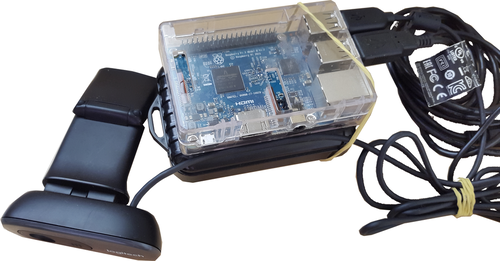
\includegraphics[width=0.66\textwidth]{imgs/berry.png}
  \caption{The Berry part of the robot.}
\end{figure}

A MicroSD with 16GB provides both the Raspbian operating system, which is based on Debian, as well
as an additional 1 GB swap memory space, as the Berry contains only 1GB RAM. The remaining amount
is used as storage.

Although the Berry has reasonable processing power for its size, training is done offline in a
desktop computer, with only inference done on the micro-computer. On the training-side computer, we
generate the SPN and then serialize it into a string of bytes and save it to a binary file. This
file is then sent through SSH to the Berry, read, loaded into memory, converting the array of bytes
into a full SPN, and then used for inference.

With its connected webcam, the Berry receives each image frame, applies some pre-processing to the
image (which will be detailed in~\Cref{chp:benchmarks}), feeds it to the SPN as evidence,
computes the most probable classification label, and finally sends this to the external unit, i.e.
the Brick, responsible for dealing with the robot's motion. This is all done concurrently, as we
can dedicate three cores to classification, and the remaining unit to camera capture, image
pre-processing and message passing.

\section{The Brick}

The Lego Mindstorms robot is composed of three main parts: the brick, which is the Lego Mindstorm's
processing unit that handles the motors, and two differential motors that are able to give motion
to the robot in a somewhat precise manner through the use of tachometers. In this document, when we
say the Brick, we are referring to the whole set of brick and motors.

In our experiments we used the Lego Mindstorms NXT. Its main processor is an Atmel AT91SAM7S256
with a 48 MHz clock and 32-bit ARMv4 architecture. It has 64 KB of RAM and 256 KB of flash storage.
A USB port allows for local input and output from and to the Brick.

\begin{figure}[h]
  \centering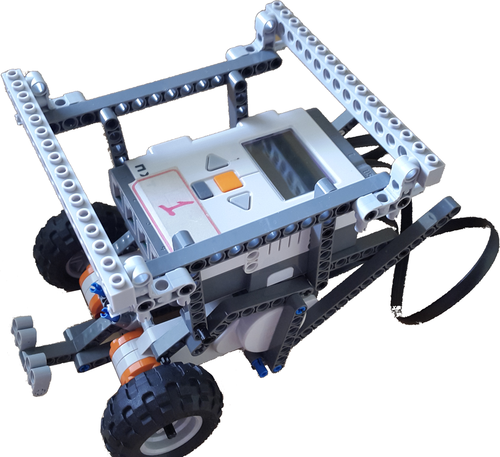
\includegraphics[width=0.66\textwidth]{imgs/brick.png}
  \caption{The Brick part of the robot.}
\end{figure}

Low-level handling is done on the Brick. Once it receives a command to be executed (i.e. the
classification label passed by the Berry), the Brick needs to interpret it and execute the desired
movement. We use the leJOS NXJ API\footnote{Available at \url{http://lejos.org/nxj.php}} for
low-level motor programming. The Brick's cycle is as follows:

\begin{algorithm}[H]
  \caption{\code{Brick}: The Brick's cycle}
  \begin{algorithmic}[1]
    \State Connect and power up motors
    \State Let \code{UP} $\gets$ \code{0x00}
    \State Let \code{LEFT} $\gets$ \code{0x01}
    \State Let \code{RIGHT} $\gets$ \code{0x02}
    \State Let \code{QUIT} $\gets$ \code{0x03}
    \State Let \code{NOOP} $\gets$ \code{0x04}
    \State Let $M_L$ and $M_R$ be the left and right side motors respectively
    \State Let $k$ be some speed constant
    \While{\textbf{true}}
      \If{input size $>$ 0}
        \State Read input byte and store in variable $c$
        \If{$c$ is \code{QUIT}}
          \State Disconnect and power down
        \ElsIf{$c$ is \code{UP}}
          \State Set $M_L$'s power to $k$
          \State Set $M_R$'s power to $k$
        \ElsIf{$c$ is \code{LEFT}}
          \State Set $M_L$'s power to $2k$
          \State Set $M_R$'s power to $3k$
        \ElsIf{$c$ is \code{RIGHT}}
          \State Set $M_L$'s power to $3k$
          \State Set $M_R$'s power to $2k$
        \EndIf%
      \EndIf%
    \EndWhile%
  \end{algorithmic}
\end{algorithm}

No complex control is done on the Brick. A standard ``do something until told otherwise'' is
implemented. This is reliant on the Berry's inference speed, but we found that inference was fast
enough for this to work well on slow speeds.

Setting the motors' power is straightforward with leJOS. Two function calls are enough for our
case. The problem is in choosing $k$. If $k$ is too big, not only the Berry might not have enough
time to compute the labels, but also turns may not be as steep as the lane requires. In the case of
a too small $k$, the challenge of autonomous driving becomes null. We experimented on values of $k$
and chose $k=150$ for our Lego Mindstorms. We recognize that a better control solution to this
would be preferred, but for our case this suffices.

\section{Bridging the two}

Communication between the two modules, Berry and Brick, is done through a USB cable. We use a Go
codebase on the Berry, opting to use Google's GoUSB\footnote{Available at
\url{https://github.com/google/gousb}} as a low-level interface to handle the Raspberry Pi's data
output, sending each predicted label as a byte value.

At each cycle, the Brick checks for new input by reading from an input stream. This is done through
Java's \code{java.io.DataInputStream}, which translates the incoming USB data into Java bytes.

This hierarchization of Berry to Brick allows for the unit with most processing power, i.e.  the
Berry, to take on the heavy load, leaving only the necessary dedicated low-level motor handling to
the Brick, a very limited processing unit in terms of power and memory.

\begin{figure}[h]
  \centering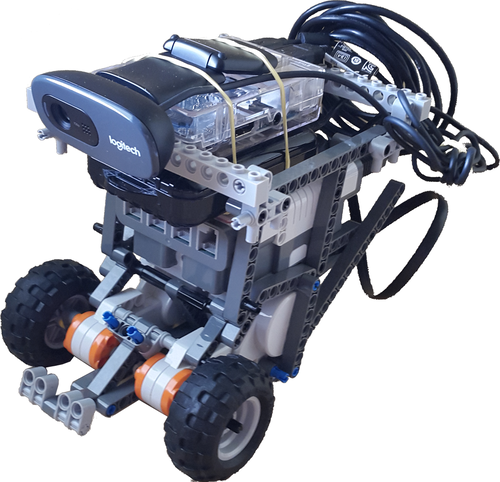
\includegraphics[width=0.66\textwidth]{imgs/robot.png}
  \caption{Fully assembled robot.}
\end{figure}

Every USB device contains a pair of IDs that are essential for identification. The vendor ID is
used to identify which company or organization created the device. Whilst the product ID is used to
identify specific products created by the company. In our case, the vendor refers to the Lego
Mindstorms company and the product to the NXT version 2, which are \code{0x0694} and \code{0x0002}
respectively.  These IDs allow us to cycle through each active USB device and select exactly the
one we need.

USB devices may contain multiple functionalities, such as acting as a power source or as an
input/output stream. These are called configurations, and are usually indexed by a number. In our
case we are interested in the read and write configuration of the Brick, indexed by the number 1.

Each configuration contains different interfaces that can be seen as virtual devices to the
physical USB. We selected interface number 0, with alternative interface 0.

When writing and reading from and to a USB device, we must define an output and input endpoint.
There are a total of 30 endpoints, where input endpoints are indexed from \code{0x81} to
\code{0x8f}, and output endpoints from \code{0x01} to \code{0x0f}. Two additional in/out endpoints
\code{0x80} and \code{0x00} are control endpoints used internally by the USB device. For our Brick
we used the input \code{0x82} and output \code{0x01} endpoints.
